%!TEX root=../document.tex

\section{Einleitung}
\subsection{Definition}
Replikation (lateinisch \textit{replicatio} \cite{duden} ``Wiederholung``, ``kreisförmige Bewegung``) \cite{dict} ist ``ein Verfahren der Datensicherung bei dem dieselben Daten von einem primären Speichermedium auf ein oder mehrere sekundäre Speichermedien kopiert werden.`` \cite{itw}

Demnach wäre Replikation also nichts anderes als ein simples Backup. Replikation wird jedoch besser definiert als mehrfache Speicherung \textbf{identer} Daten (an unterschiedlichen Orten) inklusive der Synchronisation selbiger. \cite{wiki}

Zwar gibt es inkrementelle Backups, die ebenfalls eine gewisse Synchronisierung der Daten beinhalten, jedoch erfolgt diese bei Backups stets einseitig. Bei der Replikation kann sie auch bidirektional implementiert werden. Ebenfalls wird bei einem Backup nie direkt mit den Sekundärdaten, also dem eigentlich Backup, gearbeitet, diese dienen lediglich als Absicherung im Verlustfall.

\subsection{Caching vs. Replikation}

Caching (Cache = Versteck, geheimes Lager) wird, im Unterschied zur Replikation, definiert als \textbf{temporäres} Speichern von redundanten Daten, die dynamisch ausgewählt werden. Zusätzlich sollte der Cache für die Administration möglichst unsichtbar sein, wovon bei der Replikation nicht die Rede sein kann. \cite{kaiserslautern}

\section{Pro \& Kontra}

\subsection{Gründe für Replikation}

Die Replikation ist also die bewusste Erzeugung redundanter Daten, obwohl dies eigentlich den Normalformen, die beim Planen einer Datenbank beachtet werden sollten, widerspricht. \cite{kaiserslautern} Trotzdem haben diese absichtlichen Redundanzen Vorteile:

\subsubsection{Skalierbarkeit}
\label{sec:scale}

Aufgrund mehrerer identer Datenbankinstanzen können Lesezugriffe verteilt werden. Somit wird die Last an den einzelnen Knoten reduziert und das Gesamtsystem wird dadurch leichter skalierbar. \cite{kaiserslautern}

\subsubsection{Verfügbarkeit}

Mithilfe von Replikation wird ebenfalls die Verfügbarkeit des Gesamtsystems erhöht, da im Fehlerfall eines einzelnen Knotens die Erreichbarkeit des Systems nicht beeinträchtigt wird. Andere Knoten können das System weiterhin aufrecht erhalten, womit der Extremfall ``Totalausfall`` ausgeschlossen wird. Zusätzlich gehen im Gegensatz zu einfachen verteilten Datenbanken keine Informationen verloren, sollte eine Instanz (dauerhaft) ausfallen, da alle Instanzen den identen Datensatz zur Verfügung haben. \cite{leipzig}

\subsubsection{Performance}

Replikation verbessert die Antwortzeiten auf zwei Arten:

Zuerst werden die Antwortzeiten des System verkürzt, da die Last auf mehrere Server verteilt wird. Somit haben einzelne Knoten mehr Ressourcen zur Verfügung um einem Client schneller zu antworten. Das ist der angenehme Nebeneffekt der Skalierbarkeit (Unterpunkt \ref{sec:scale} auf Seite \pageref{sec:scale}). \cite{leipzig}

Zusätzlich werden die lokalen Antwortzeiten des System verkürzt, da stets auf eine ortsnahe oder netztopologisch günstige Instanz der Datenbank zugegriffen wird. \cite{leipzig}

\begin{figure}[!h]
	\begin{center}
		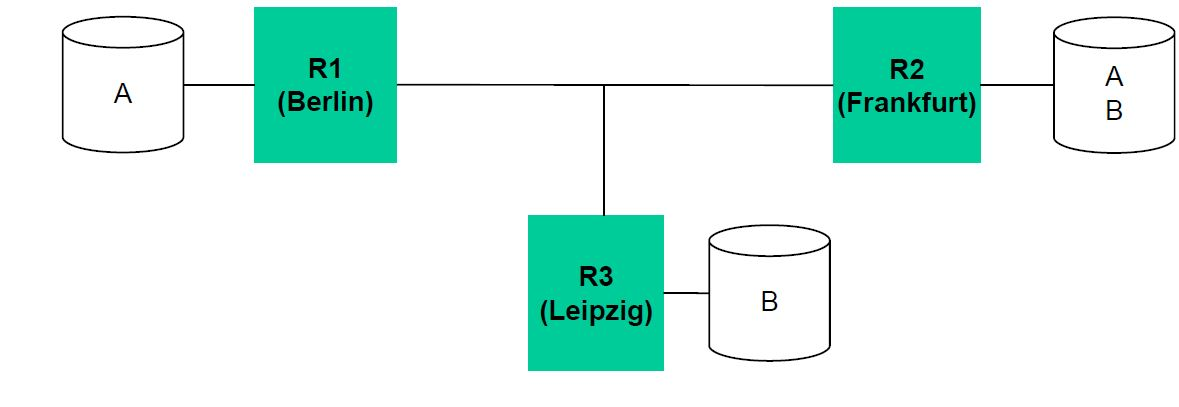
\includegraphics[width=1\linewidth]{images/ortsverteilung.jpg}
		\caption{Replikate an verschiedenen Standorten \cite{leipzig2}}
		\label{ortsvert}
	\end{center}
\end{figure}

Die verbesserten Antwortzeiten gelten meist nur für Lesezugriffe, da Schreibzugriffe in der Regel nicht vollkommen autonom ablaufen können. Dazu später mehr.

\subsubsection{Disconnected Computing}

Clients können ausgewählte Daten lokal replizieren, um damit später offline zu arbeiten. Im Anschluss müssen die Daten des lokalen Replikats mit den anderen Instanzen synchronisiert werden. \cite{leipzig} Die replizierten Daten sind in diesem Fall zwar meist nur temporär gespeichert, was eher auf die Funktion eines Caches hinweisen würde, jedoch wurden die zu replizierenden Daten im Vorhinein bewusst ausgewählt und im Anschluss werden sie wieder synchronisiert.

\subsection{Nachteile}

Für statische Daten sind die genannten Vorteile leicht mittels Replikation zu erreichen. Sollten sich die Daten ändern, müssen die Änderungen an alle Instanzen weitergegeben werden. Bei stark dynamischen Daten entstehen damit mehr Probleme, als gelöst werden. Deshalb wird Replikation typischerweise bei Stammdaten eingesetzt. \cite{kaiserslautern}
\clearpage
Durch die Synchronisation entstehen folgende Probleme:

\subsubsection{Aufwand}

Durch die benötigte Synchronisation der einzelnen Knoten wird das Netzwerk zwischen den Servern zusätzlich belastet. Eine Änderung an einem Knoten muss letztendlich an alle propagiert werden, weshalb der Rechenaufwand und die Netzauslastung bei stark dynamischen Daten schnell zum Problem werden.

\subsubsection{Speicherplatzbedarf}

Die vielen Instanzen benötigen insgesamt logischerweise mehr Speicherplatz, womit die Kosten für das Gesamtsystem wesentlich ansteigen. Aufgrund der Replikation ist die Menge der Informationen trotz erhöhten Speicherbedarfs gleich. Deshalb sollten die Gesamtsysteme so konzipiert werden, dass die zu replizierenden Daten der einzelnen Knoten sinnvoll ausgewählt werden.

Beispielsweise werden in der Zentrale in Frankfurt alle Datensätze benötigt. In Berlin benötigt eine andere Filiale derselben Firma nur einen Teil der Daten. In Leipzig wird wiederum nur ein anderer Teil der Daten benötigt (siehe Abbildung \ref{ortsvert} auf Seite \pageref{ortsvert}).

\subsubsection{Komplexität}

Mit der Anzahl der Knoten wächst auch die Komplexität des Gesamtsystems. Dadurch wird die Installation, Konfiguration und Wartung des Systems aufwendiger, was wiederum zu erhöhten Kosten führt.

\section{Anwendungsszenarien}

\section{Asynchrone \& synchrone Replikation}

\subsection{Konvergenz}

\section{Unidirektionale \& bidirektionale Replikation}

\section{Klassifikation}

\section{Resümee}